
\section{Data Production Department }\label{sec:sciops} \label{sec:dataprod}

The role of data production within \gls{LSST} is to deliver \gls{LSST}'s science products: the science images, the alert stream, the annual data releases, the science \gls{software}, and the Science Platform. In the current ops proposal not all groups required to do this are under control of Science operations.

\figref{fig:opsorg} gives a view of the Data Production teams which combine some of the old science operations  and LDF departments. This is far more analogous to Data Management moving into operations than in the current proposal and would make for a smoother transition.

\begin{figure}
\begin{center}
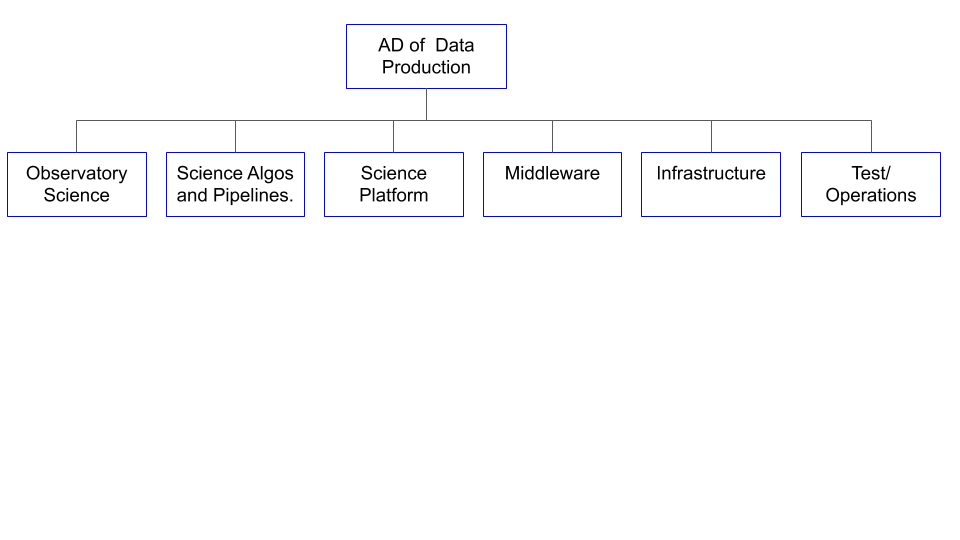
\includegraphics[width=0.9\textwidth]{figures/SciOpsOrg}
\caption{Possible configuration of Science Operations Department for operations of \gls{LSST} \label{fig:sciopsorg}}
\end{center}
% original https://docs.google.com/presentation/d/1wIN6Dj_rPn8TASBUkAm6_-Yh255Gz9VbwFi61t4LCFs/edit#slide=id.g55f7c0247e_0_2
\end{figure}

The FTE counts are estimated in \tabref{tab:FTE}.
 \begin{longtable} { |p{0.3\textwidth}  |r  |r  |r  |r |} 
\caption{Size (in FTE) of the various teams in data production department with sizes including LDF teams from the proposal in the fourth column - a zero imples the team did not exist inthe proposal. \label{tab:FTE}}\\ 
\hline 
\textbf{Team}&\textbf{2023}&\textbf{2026}&\textbf{2023(P)}&\textbf{Note} \\ \hline
{Management (AD)}&{1.5}&{1.5}&{1}& \\ \hline
{Observatory Science }&{5.5}&{5.5}&{5.5}&{System performance?} \\ \hline
{Science Platform}&{6}&{6}&{6.5}& \\ \hline
{Science Algos and Pipelines}&{22}&{16}&{21}&{QA  to system performance?} \\ \hline
{Middleware}&{7.5}&{6.5}&{0}& \\ \hline
{Infrastructure}&{8}&{7}&{0}&{ } \\ \hline
{Verification/ Operations}&{5}&{4}&{0}& \\ \hline
{LDF Management (AD) }&{0}&{0}&{3}&{In infrastruture} \\ \hline
{LDF Scientific Prod. Services}&{0}&{0}&{6.75}&{In Verification/ operations} \\ \hline
{LDF ITC Security}&{0}&{0}&{8.5}&{Some in infrastructure/ middleware } \\ \hline
{LDF Prod. Services Soft.}&{0}&{0}&{7.6}&{Some in infrastructure} \\ \hline
{LDF ITC and Facilities}&{0}&{0}&{13}&{Should be in services charges} \\ \hline
\textbf{Total  FTE}&\textbf{55.5}&\textbf{46.5}&\textbf{72.85}& \\ \hline
\end{longtable}


\subsection{Teams }\label{sec:teams}
\figref{fig:sciopsorg} introduces several teams some of which were not in the original ops proposal. I  little detail is given here about each.

\subsubsection{Observatory Science}
As in the ops proposal the primary responsibility of this team is to understand the end-to-end impact of the Observatory hardware and environment on the science images and to work with the Observatory Operations department to ensure that the image quality meets requirements.

\textbf{This team may be better  in Observatory operations department }

\subsubsection{Science algorithms and pipelines}
This team is responsible to assess and assure the alert stream and annual data releases.
In the submitted proposal this includes extensive \gls{QA} to compare the data products against requirements -
this may be be better merged with Sytem Perfomance/Verification.
The main responsibility  of this team  would then be the  underlying \gls{software} pipelines themselves. Monitoring and updating the calibration plan and algorithmic implementation is also a responsibility of this team. The Calibration Support Scientist on the Observatory Science team will be responsible for monitoring the physical implementation of the calibration plan at the summit.
In \tabref{tab:FTE} this team is initially sized similarly to the AP/DRP teams in construction. There will be signifcant maintenance in the first two or three years of operations. As mentioned above there may be some consolidation with \gls{QA} activites in System Performance.

\subsubsection{Science platform  }
This team will be responsible for maintaining and evolving LSST’s user access portal, the Science Platform. This will include keeping up with evolving technologies and computing infrastructure, as well as providing basic code-base maintenance, bug fixes, and low-level response to science community and internal \gls{LSST} requests for new features.

\subsubsection{Middleware }
In a service oriented model with a layered architecture as outlined in \secref{sec:arc} it is essential to have a cross cutting team who compose and debug services.
Software such as the \texttt{butler}  is not part of the pipeline but the pipeline needs it. In house developments such as \gls{Qserv} should be covered here (1.5FTE has been included f0r this - DOE/SLAC personnel - could be 2).
This would also cover the builds and how the code interacts with the infrastructure (\secref{sec:infra}.

\subsubsection{Infrastructure, Site Reliability Engineering  } \label{ses:infra}
This is for deployment of of various systems and pipelines. Configuration is included in this. There needs to be a couple of people who manage keys/secrets
for access to commodity services. We would need a security resource as well as database expertise.  This then implies using tooling for system management as
provided by e.g. \gls{AWS} console.

In general an \gls{SRE} team is responsible for the availability, latency, performance, efficiency, change management, monitoring, emergency response and capacity planning of their services \cite{Beyer:2016:SRE:3006357}.

This team would include paying for a liaison at any service provider e.g. Google Professional Services or a Service Manager at \gls{NCSA}. (2FTE calculated)

\subsubsection{Verification/Operations }
This team will take and verify new releases for operations before they are deployed to the operations system. They will monitor the operational system to make sure it is functioning - they should have some science knowledge to know it is actually working properly as opposed to not just giving errors. A team of 4 should be able to handle this.
Some support for this is assumed from IN2P3 .




\subsection{Other implied changes to the current operations proposal}
Notably missing from \figref{fig:sciopsorg} is \gls{QA}. Currently \gls{QA} is spread across  three
 departments - the suggestion here is to place all \gls{QA} activities under the survey performance department. Consolidation
of the \gls{QA} activities in one department may allow for some personnel saving.

The data release team in science operations would require a verification scientist (this may be 0.5FTE) while the \gls{SDQA} and Semantic scientists may move to QA in survey science.

All data facility work, be it with a partner or in commercial \gls{cloud} should be firmly under science operations - hence there is no LDF department and no associate director for LDF as depicted in \figref{fig:opsorg}.\footnote{This is  in line with AMCL recommendations}


\begin{figure}
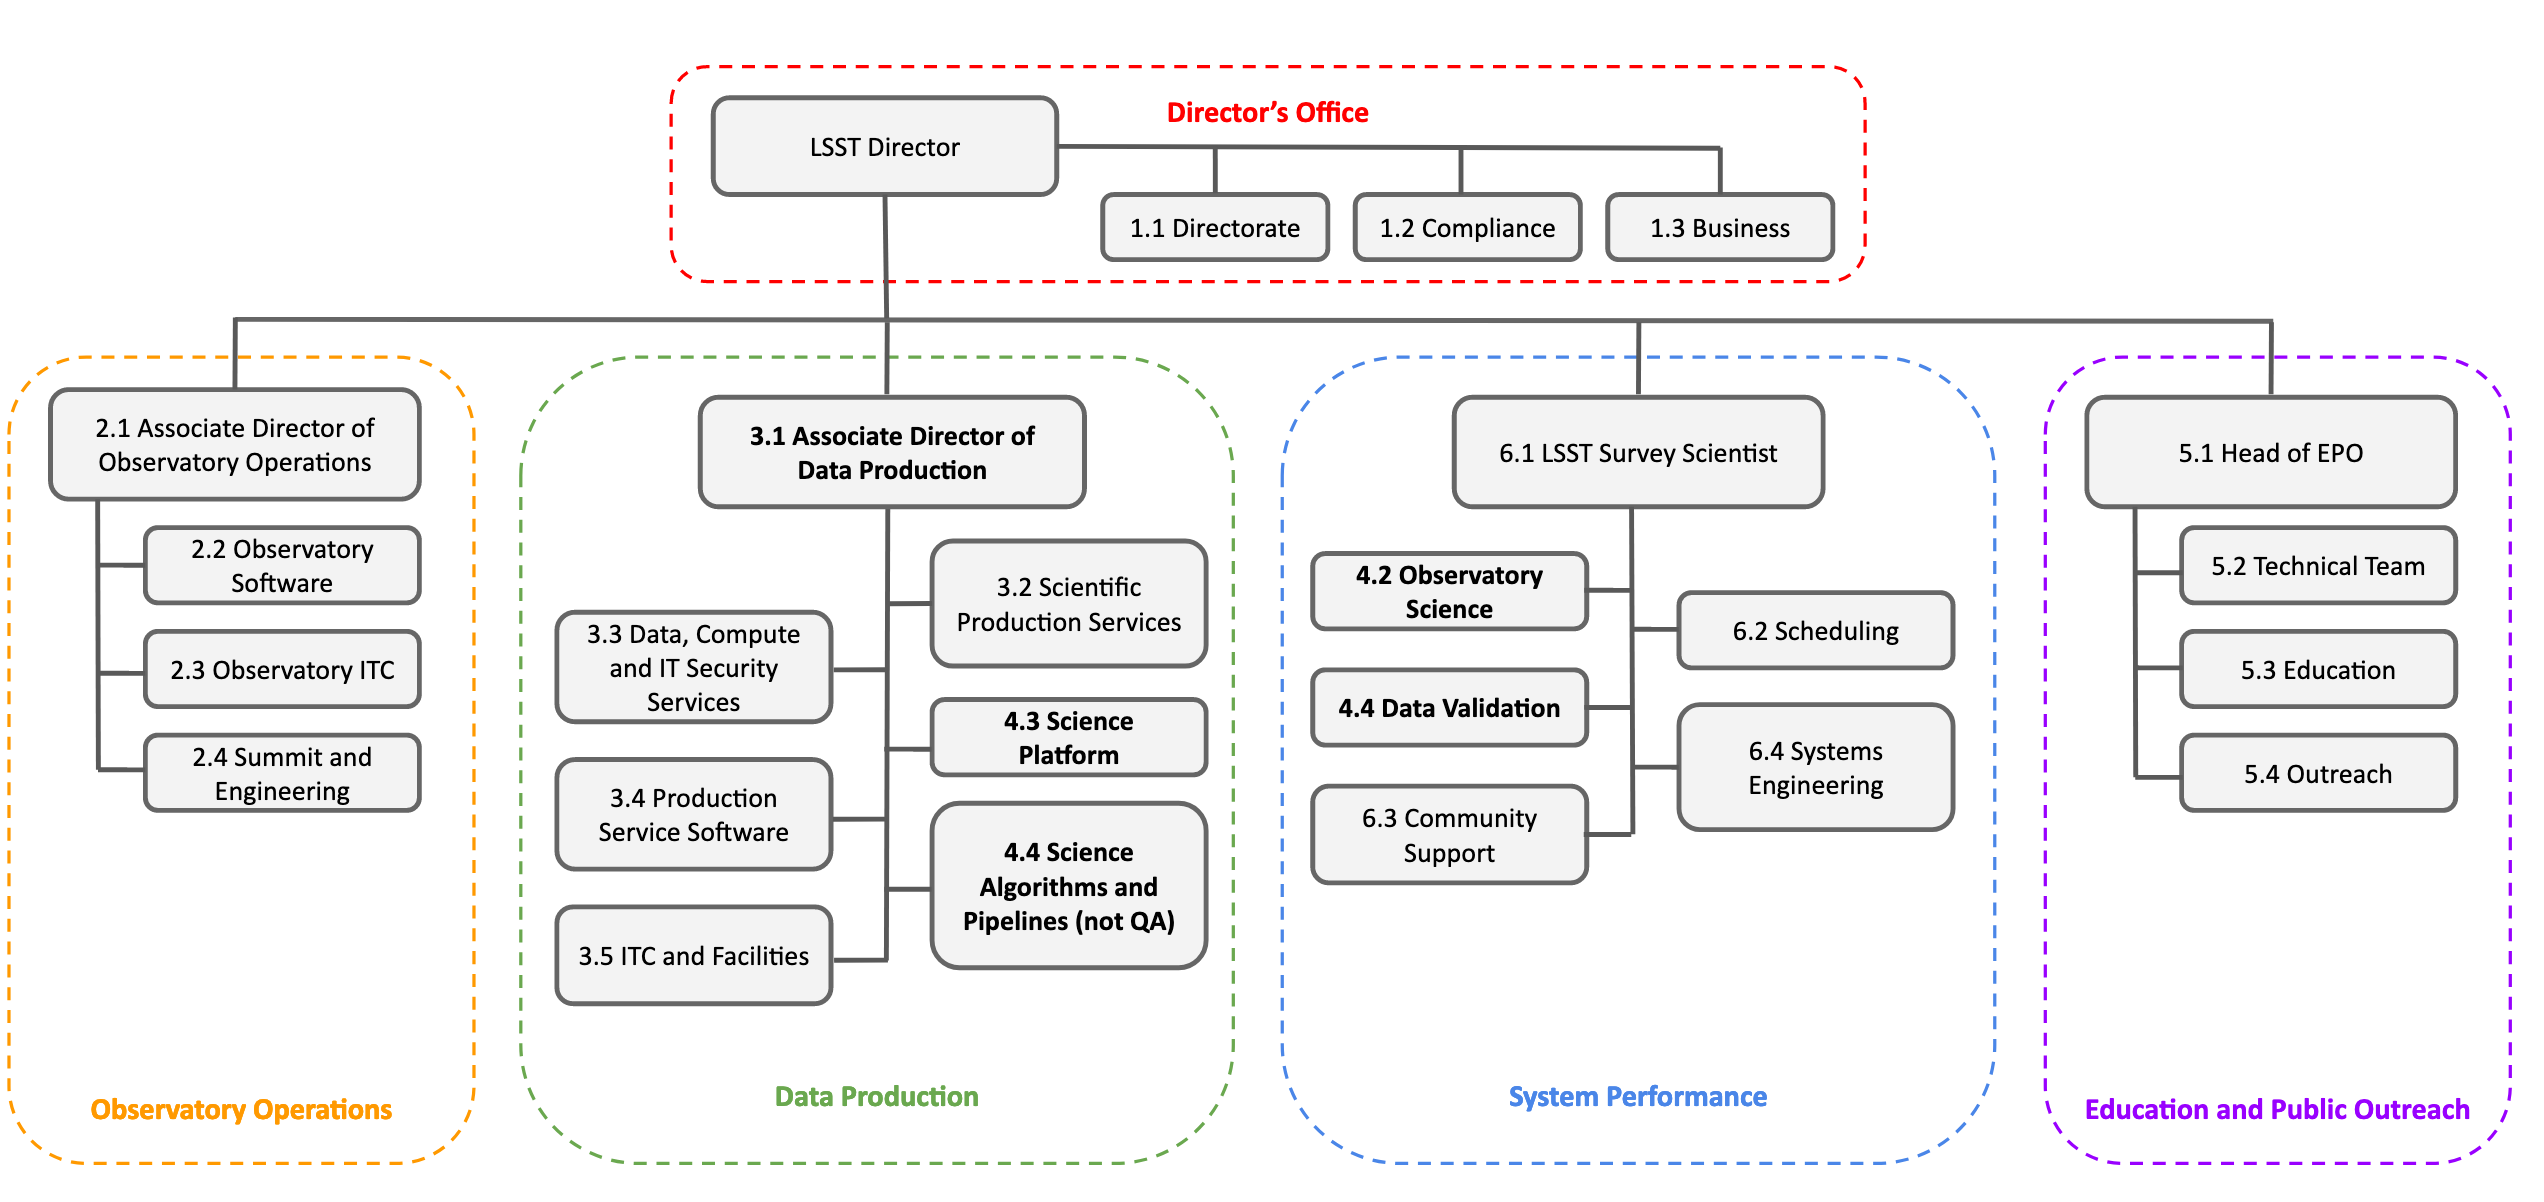
\includegraphics[width=1.0\textwidth]{figures/OpsOrg}
\caption{Possible new organisation chart for \gls{LSST}  operations \label{fig:opsorg}}
% original https://docs.google.com/presentation/d/1H7sn92FXDa9-cgFrizgN12KI3Br60Ffbk4qA8fxCvMg/edit#slide=id.g5132af8469_0_81
\end{figure}

\textbf{NOTE: I have said before communications should report directly to the director - in \figref{fig:opsorg} there is NO communications.}

ITC and facilities (\figref{fig:opsorg}) in this model should come from NCOA  logically also this does not belong in data production but at a higher level its for the entire org, the observatory already has its own ITC group so they are good.

